%%This is a very basic article template.
%%There is just one section and two subsections.
\documentclass{article}

\usepackage{hyperref}
\usepackage{listings}
\usepackage{graphicx}
\usepackage{caption}
\usepackage{subcaption}
\usepackage{tikz}

% "define" Scala
\lstdefinelanguage{scala}{
  morekeywords={abstract,case,catch,class,def,%
    do,else,extends,false,final,finally,%
    for,if,implicit,import,match,mixin,%
    new,null,object,override,package,%
    private,protected,requires,return,sealed,%
    super,this,throw,trait,true,try,%
    type,val,var,while,with,yield},
  otherkeywords={=>,<-,<\%,<:,>:,\#,@},
  sensitive=true,
  morecomment=[l]{//},
  morecomment=[n]{/*}{*/},
  morestring=[b]",
  morestring=[b]',
  morestring=[b]"""
}

\lstset{ 
  breaklines=true,         % sets if automatic breaks should only happen at whitespace
  postbreak=\raisebox{0ex}[0ex][0ex]{\ensuremath{\hookrightarrow\space}},
  language=scala
}

\begin{document}
\title{Pushing down arbitrary logical plans}
%\author{Stephan Kessler
%(\href{mailto:stephan.kessler@sap.com}{stephan.kessler@sap.com})}
\maketitle

\section{Motivation}

The DataFrame API of Spark SQL allows the easy integration of external sources such as SQL Databases, CSV files or Avro sources. In addition to this, Spark uses the computational capabilities of data sources to ‘push­down’ projections as well as filters to the data source. This prunes unnecessary data right in the source, reducing evaluation time on Spark level. However, sources such as SQL Engines also allow the evaluation of more complex parts of the logical plan. Enabling such capabilities of the sources allows for a huge performance boost: For example, evaluating aggregates or joins directly in the source, reduces the amount of copied data dramatically. In this document, we propose an extension to the Spark API and explain a possible implementation.

\section{Implementation}

The implementation consists of two parts: First, a new interface for the data sources that are able to process a full or at least a part of the logical plan, and second, an integration into physical planning. In the following, we explain our design decisions. 

\subsection{The CatalystSource Interface}

We propose the following \textit{CatalystSource}-interface, that is implemented by data sources that can process logical plans.

\begin{lstlisting}[frame=single]
trait CatalystSource {
 def supportsLogicalPlan(plan: LogicalPlan): Boolean
 def isMultiplePartitionExecution(relations: Seq[CatalystSource]): Boolean
 def logicalPlanToRDD(plan: LogicalPlan): RDD[Row]
}
\end{lstlisting}

Even though we assume we have a data source that is capable of doing sophisticated data processing, i.e., a SQL engine, we still cannot make any assumption if a specific logical plan is supported. The method \textit{supportsLogicalPlan} returns a boolean value, indicating whether the data source can process such a plan or not --- if not, SparkSQL will take care of at least a part of it. 

A data source could either be partitioned or holistic. \textit{Partitioned} means that a separated data source instance runs on parallel on each or some cluster nodes and each of the instances is only holding a fraction of the data (see Fig.~\ref{fig:partitionedDS}). \textit{Holistic} means the data source runs completely separated as a single instance containing all the data (see Fig.~\ref{fig:holisticDS}). 

In case the execution involves multiple partitions, Spark has to take care of the following things during physical planning:
\begin{itemize}
  \item[a)] merging the results, e.g., aggregates and
  \item[b)] global operations such as DISTINCT. 
\end{itemize}
  
This depends on the relations required, e.g., relations could be co-partitioned or belong to different kind of data sources. Thus, a data source also must have the ability to report back to Spark if it requires a partitioned execution. The method \textit{isMultiplePartitionExecution} returns true if the execution has to be partitioned, and false if it is holistic for the given relations. 

When a data source is able to process a logical plan, it has to be converted to an RDD for physical planning. The method \textit{logicalPlanToRDD} implements that functionality.

\begin{figure}
\centering
\begin{subfigure}{.5\textwidth}
  \centering
  \includegraphics[width=0.9\textwidth]{images/partitionedDS.png}
  \caption{Partitioned Datasource}
  \label{fig:partitionedDS}
\end{subfigure}%
\begin{subfigure}{.5\textwidth}
  \centering
  \includegraphics[width=0.9\textwidth]{images/holisticDS.png}
  \caption{Holistic Datasource}
  \label{fig:holisticDS}
\end{subfigure}
\caption{Different kinds of Datasources for the CatalystSource Interface}
\label{fig:partitionedVsHolistic}
\end{figure}

\subsection{Integration into physical planning}

In order to incorporate the \textit{CatalystSource} datasources, we add another strategy to the physical planner, \textit{CatalystSourceStrategy}. This strategy implements the following logic when applied to a logical plan \textit{p}:

\begin{enumerate}
  \item If there is no relation in \textit{p} that is implementing the \textit{CatalystSource} interface, the strategy returns \textit{Nil} since it is not applicable, else it continues.
  \item The strategy determines if it is a partitioned or a holistic execution by calling the \textit{isMultiplePartitionExecution} method on one of the \textit{CatalystSource}s. (Note: Each of them returns the same boolean value.) Next steps depend on the result:
  	\begin{itemize}
  		\item \textbf{Holistic Execution:} The strategy returns a \textit{PhysicalRDD} containing the resulting attributes and the RDD returned by \textit{logicalPlanToRDD(p)}.
  		\item \textbf{Partitioned Execution:} During the partitioned execution, global operations (LIMIT, SORT, DISTINCT, INTERSECT, EXPECT, AGGREGATE) cannot be executed in a \textit{CatalystSource}. If the logical plan contains such a global operation, the resulting physical plan contains a sequence of the physical RDD for the global operation followed by the resulting RDD returned by \textit{logicalPlanToRDD(p.child)}. Note: If \textit{p.child} still contains global operations, planning returns \textit{Nil}. 
	\end{itemize}
	\item If the data sources do not support the logical plan or if planning is not possible, this strategy will return \textit{Nil}. If other planning strategies decide that a certain subtree should be planned later, it gets called again. For instance, this is the case for Joins, where both subtrees are planned later.
\end{enumerate}

\section{Example}

For illustrative purposes, we provide an example. This example is similar to the one presented at Spark Summit Europe 2015\footnote{\url{https://spark-summit.org/eu-2015/events/the-pushdown-of-everything/}}. 

Assume there is a table \textit{attendees} with three columns: \textit{Name} as String, \textit{Age} as Integer and \textit{Hometown} as String column (see Table~\ref{tab:exampleData}).

\begin{table}[htb]
\centering
	\begin{tabular}{ l | l | l }
  		\textbf{Name} & \textbf{Age} & \textbf{Hometown} \\
  		\hline
  		Peter & 23 & London \\
  		\hline
  		John & 30 & Amsterdam \\
  		\hline
  		Stephan & 72 & Karlsruhe \\
  		\hline
  		\ldots & \ldots & \ldots \\
	\end{tabular}
	\caption{Example Data Set, Table \textit{attendees}}
	\label{tab:exampleData}
\end{table} 

The user tries to receive the average age of attendees coming from `Amsterdam', in SQL: 

\begin{lstlisting}[frame=none,language=sql]
SELECT Hometown, AVG(Age) FROM attendees 
  WHERE Hometown = 'Amsterdam' 
  GROUP BY Hometown
\end{lstlisting}

If the data source requires \textit{partitioned execution}, i.e., the table is partitioned over multiple instances, part of the `average' query has to be executed on Spark level, while `sum' and `count' are executed in the data source to do a pre-aggregation, see Figure~\ref{fig:partitionedExecution}.

\begin{figure}[htp]
\centering
  \includegraphics[width=1.0\textwidth]{images/partitionedExecution.png}
  \caption{Partitioned Execution, dark orange part is executed in the data source, SQL part only for illustration}
  \label{fig:partitionedExecution}
\end{figure}

Otherwise, if the data source requires \textit{holistic execution}, the complete query is executed in the datasource, and the result does not require further processing, see Figure~\ref{fig:holisticxecution}.

\begin{figure}[htp]
\centering
  \includegraphics[width=1.0\textwidth]{images/holisticExecution.png}
  \caption{Holistic Execution, dark orange part is executed in the data source, SQL part only for illustration}
  \label{fig:holisticxecution}
\end{figure}

Implications for performance are as follows: Evaluating aggregates directly at the source minimizes data transfer between the source and Spark. In this case, only one row is transferred from each source partition to Spark. The number of returned rows for a data source implementing \textit{PrunedFilterScan}-interface depends on the data set, i.e., the number of rows where \textit{homewtown = `Amsterdam'}.

\section{Gradual Approach}

Pushing down logical plans as proposed before has the major drawback that the logical plan API has to be rather stable. Thus, we strive for a different approach not exposing the logical plan api.

Design goals are as follows:

\begin{itemize}
  \item The API of the pushed down elements can stay stable, while the logical plan api might change
  \item We add the ability to push down  operations such as aggregates. Mechanism has to be extendable to all elements of the logical plan.
  \item The set of operations that can be pushed down depends on the datasource, i.e., a datasource could support a subset of the possibled pushed down operations.
\end{itemize}



\subsection{Current Approach for Filters and Projections}

The current push down is controlled by the \textit{DataSourceStrategy}, there are two code paths involving Projections and Filters. Depending on the capabilities of the datasource, it has to implement different traits (\textit{PrunedScan,PrunedFilterScan})

\textit{Projections} are currently pushed down by providing the named columns as a String, see the \textit{PrunedScan} trait.

\begin{lstlisting}[frame=none,language=scala]
@DeveloperApi
trait PrunedScan {
  def buildScan(requiredColumns: Array[String]): RDD[Row]
}
\end{lstlisting}

For \textit{Filters} this is slightly different. The \textit{PrunedFilterScan} Interface requires an array containing elements of type \textit{Filter}. 

\begin{lstlisting}[frame=none,language=scala]
@DeveloperApi
trait PrunedFilteredScan {
  def buildScan(requiredColumns: Array[String], filters: Array[Filter]): RDD[Row]
}
\end{lstlisting}

Expressions are converted by the function \textit{translateFilter} which is called by the \textit{DataSourceStrategy}.

\subsection{Extending the Approach for Complex Parts}

We need to consider two parts: First, how could we abstract the logical plan from actually pushed down operations such that we do not expose internal API. Second, we require a more flexible pushdown mechanism that reflects the datasource capabilities.

\subsubsection{Abstraction of the logical plan}

Following the already existing logic of creating new case classes for pushed down filters, we abstract that principle. Every operation that can be pushed down inherits the trait (or abstract class) \textit{LogicalPlanOperation}. The already existing class \textit{Filter} also has to inherit this new marker trait. See Figure~\ref{fig:inheritanceLogicalPlanOperation} for in illustration of the inheritance hierarchy.

\begin{figure}
\centering
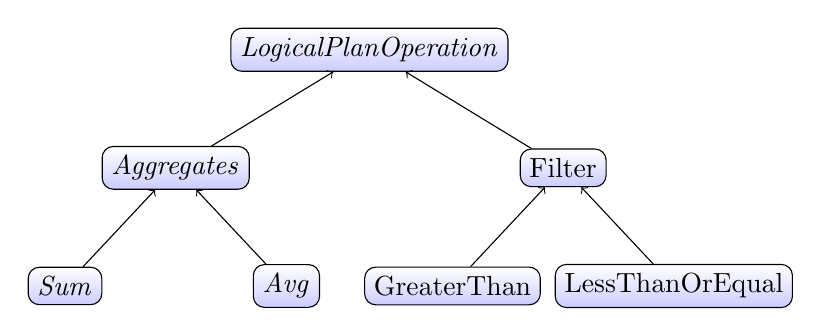
\begin{tikzpicture}[<-,
  every node/.style = {shape=rectangle, rounded corners,
    draw, align=center,
    top color=white, bottom color=blue!20}]]
    \tikzstyle{level 1}=[sibling distance=14em]
    \tikzstyle{level 2}=[sibling distance=8em]
  \node[fill=blue!20] {\textit{LogicalPlanOperation}}
    child { node[fill=blue!20] {\textit{Aggregates}} 
    	child { node[fill=blue!20] {\textit{Sum}}}
    	child { node[fill=blue!20] {\textit{Avg}}}
    }
    child { node {Filter} 
      child { node {GreaterThan} }
      child { node {LessThanOrEqual} } 
      };
\end{tikzpicture}
\caption{Inheritance including new \textit{LogicalPlanOperation} trait, Blue nodes represent new classes/interfaces} 
\label{fig:inheritanceLogicalPlanOperation}
\end{figure}

For every operation that finally should become a \textit{LogicalPlanOperation} and thus can be pushed down, we require a translation step inside the \textit{DataSourceStrategy} which decouples the API of the logical plan from the `pushed down operations API'.

\subsubsection{Pushdown mechanism}

We propose the following \textit{ComplexDataSource} interface that a data source has to implement to retrieve \textit{LogicalPlanOperations}.

\begin{lstlisting}[frame=single,language=scala]
trait ComplexDataSource {
 def supportsLogicalPlanOperations(ops: Seq[LogicalPlanOperations]): Boolean
 def logicalPlanToRDD(ops: Seq[LogicalPlanOperations]): RDD[Row]
}
\end{lstlisting}

During the physical planning, the operations have to be pushed down. The logic for that is as follows:

\begin{enumerate}
  \item Identify a part of the tree that can be translated and pushed down. This part has to satisfy the following conditions: 1) Contains only operations that have a representative as an \textit{LogicalPlanOperation} 2) Its only leaf is a \textit{ComplexDataSource}.
  \item Translate the subtree (by definition of the first step it is a path, so technically a sequence) in a sequence of \textit{LogicalPlanOperations}
  \item Ask the datasource if it is capable of processing that sequence (call \textit{supportsLogicalPlanOperation}), if yes call the \textit{logicalPlanToRDD} method and replace the subtree with the newly created RDD.
\end{enumerate}

\paragraph{Example}

Assume a datasource supports the pushdown of \textit{sum} but not of the \textit{avg} aggregate and all the filters and projects. Following the logic explained in the paragraph before, the more elements can be pushed down for the Logical Plan in Figure~\ref{fig:pushingDownSum} than in Figure~\ref{fig:notPushingDownAvg}.

\begin{figure}
\centering
\begin{tikzpicture}[<-,  every node/.style = {shape=rectangle, rounded corners,
    draw, align=center,
    top color=white, bottom color=blue!20}]]
    \tikzstyle{level 1}=[sibling distance=4em,level distance=3em]
  \node[fill=blue!20] {OP1} 
    child { node[fill=yellow!20] {Filter $sum > 20$}
   	 child { node[fill=yellow!20] {Sum(x) GroupBy(y) as sum}
    	child { node[fill=yellow!20] {Project x,y}
    		child { node[fill=grey!20] {ComplexDataSource(x,y,z)}
    			}	
    		}
    	}
    };
\end{tikzpicture}
\caption{Pushdown example, yellow nodes can be translated and pushed to the datasource} 
\label{fig:pushingDownSum}
\end{figure}

\begin{figure}
\centering
\begin{tikzpicture}[<-,  every node/.style = {shape=rectangle, rounded corners,
    draw, align=center,
    top color=white, bottom color=blue!20}]]
    \tikzstyle{level 1}=[sibling distance=4em,level distance=3em]
 \node[fill=blue!20] {OP1} 
    child { node[fill=blue!20] {Filter $avg > 20$}
   	 child { node[fill=blue!20] {Avg(x) GroupBy(y) as avg}
    	child { node[fill=yellow!20] {Project x,y}
    		child { node[fill=grey!20] {ComplexDataSource(x,y,z)}
    			}	
    		}
    	}
    };
\end{tikzpicture}
\caption{Pushdown example, yellow nodes can be translated and pushed to the datasource} 
\label{fig:notPushingDownAvg}
\end{figure}

\paragraph{Aliasing, Naming, etc.}

In the current implementation names of columns where only strings. However, if we also allow aliases (e.g., for aggregates) we should also push down proper attribute references. This could be done by defining a (stable) case class and inheriting \textit{LogicalPlanOperation} or by using the already defined expressions.

\end{document}
